\section{Our Approach}

\subsection{Core Pig Latin Features}
\begin{frame}{Core Pig Features}
\begin{itemize}
	\item \textbf{Programs specify queries over relations:} Designed to
	concisely facilitate common data transformation tasks.
	\item \textbf{Programs manipulate aggregate non-atomic types:} e.g. bags
	and tuples.
	\item \textbf{Programs use UDFs from environment.}
	\item \textbf{Programs specify data flow via statements:} A sequence of
	statements define dependencies between queries via var assignments and uses.
	\item \textbf{Programs are parallelizable/distributable:} Part of a long
	history in data flow and query-oriented programming.
\end{itemize}
\end{frame}

\subsection{Formalism}
\begin{frame}{Four Stages of Pig Programs}
\begin{itemize}
	\item A Pig Latin program passes through four stages of compilation:
	\begin{itemize}
		\item Logical Plan Formalism (1-1 with Pig Latin Prog)
		\item Physical Plan Formalism
		\item Map Reduce Formalism
	\end{itemize}
\end{itemize}
\end{frame}

\subsection{Formalism for Logical Plan}

\begin{frame}{Formalism for Logical Plan}
\begin{itemize}
	\item We have hope to create formalisms at each level which reflect all five
	core features.
	\item We present our first attempt of a logical plan grammar and static
	semantics
	\item We believe this reflects 4/5 core features.
\end{itemize}
\end{frame}

\begin{frame}{Conventions}
\centering
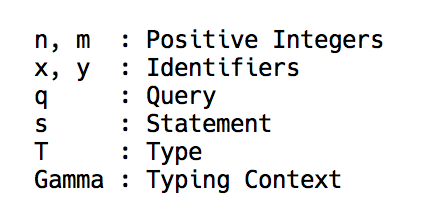
\includegraphics[scale=0.80]{conventions}
\end{frame}

\begin{frame}{Grammar: Queries}
\centering
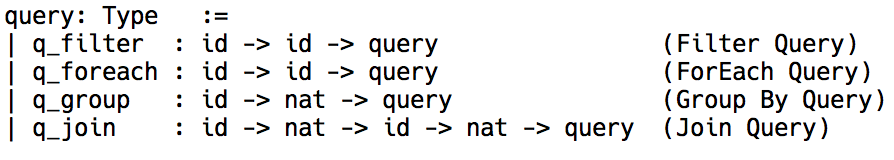
\includegraphics[scale=0.60]{query}
\end{frame}

\begin{frame}{Grammar: Statements}
\centering
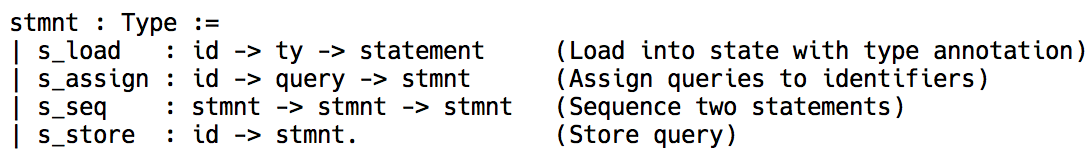
\includegraphics[scale=0.60]{stmnt}
\end{frame}

\begin{frame}{Types}
\centering
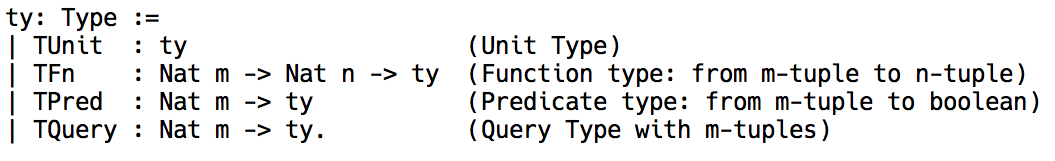
\includegraphics[scale=0.60]{ty}
\end{frame}

\begin{frame}{Typing Rules: Queries}
\centering
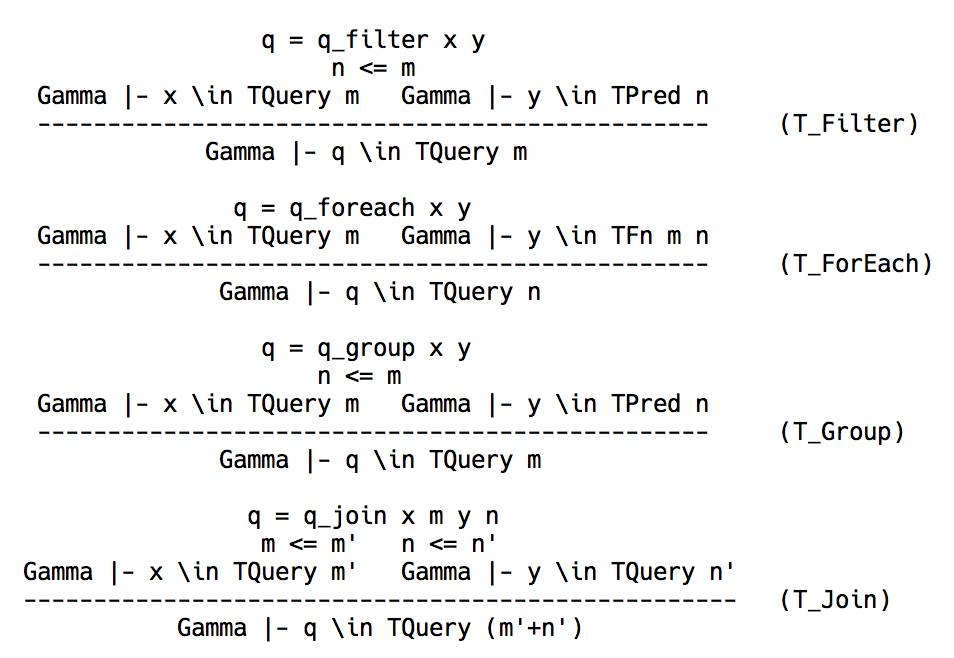
\includegraphics[scale=0.50]{T_Queries}
\end{frame}

\begin{frame}{Typing Rules: Statements}
\centering
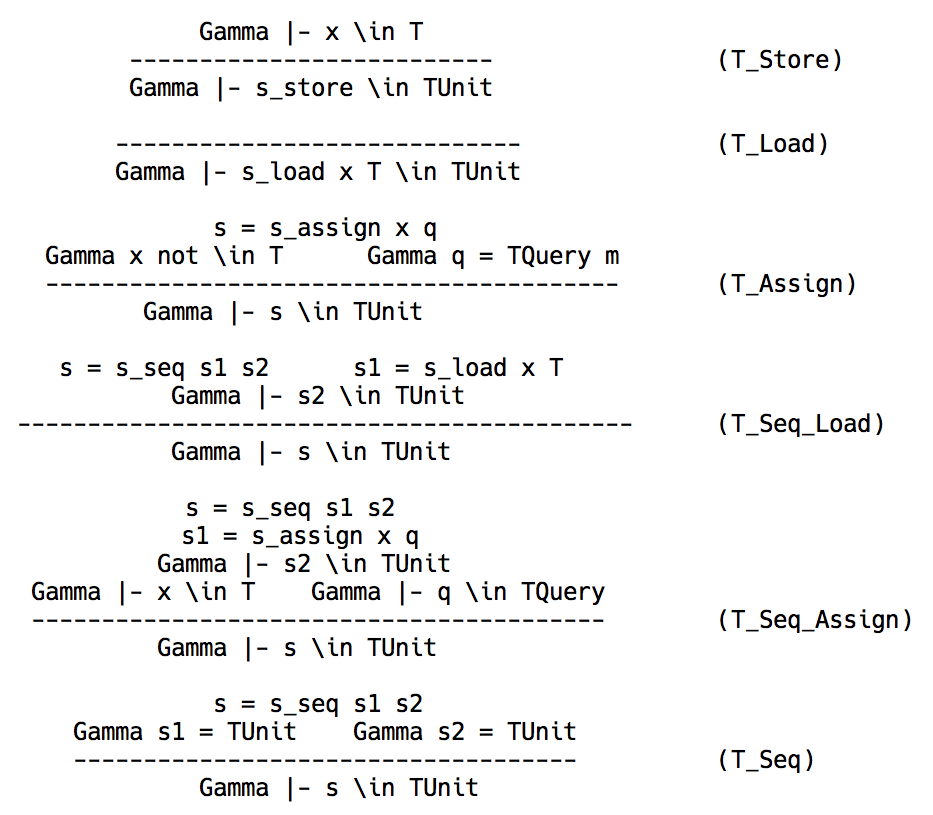
\includegraphics[scale=0.40]{T_Statements}
\end{frame}
